%%
%% This is file `./samples/longsample.tex',
%% generated with the docstrip utility.
%%
%% The original source files were:
%%
%% apa7.dtx  (with options: `longsample')
%% ----------------------------------------------------------------------
%% 
%% apa7 - A LaTeX class for formatting documents in compliance with the
%% American Psychological Association's Publication Manual, 7th edition
%% 
%% Copyright (C) 2019 by Daniel A. Weiss <daniel.weiss.led at gmail.com>
%% 
%% This work may be distributed and/or modified under the
%% conditions of the LaTeX Project Public License (LPPL), either
%% version 1.3c of this license or (at your option) any later
%% version.  The latest version of this license is in the file:
%% 
%% http://www.latex-project.org/lppl.txt
%% 
%% Users may freely modify these files without permission, as long as the
%% copyright line and this statement are maintained intact.
%% 
%% This work is not endorsed by, affiliated with, or probably even known
%% by, the American Psychological Association.
%% 
%% ----------------------------------------------------------------------
%% 
\documentclass[man]{apa7}

\usepackage[american]{babel}

\usepackage{csquotes}
\usepackage[style=apa,sortcites=true,sorting=nyt,backend=biber]{biblatex}
\usepackage{minted}
\DeclareLanguageMapping{american}{american-apa}
\addbibresource{experiment-proposal.bib}

% ellipses (three dots) in quatations definitions from: https://walden-family.com/public/texland/ellipses.pdf
    %dots for main text
    \def\bigdotsspace{3pt}
    %three dots
    \def\mydots{\hbox{\hspace{\bigdotsspace}.\hspace{\bigdotsspace}.\hspace{\bigdotsspace}.\hspace{\bigdotsspace}\hspace{\bigdotsspace}}}
    %I like the same size space on each side of the ellipsis as
    % is between the dots of the ellipsis
    
    \hypersetup{
        nolinks=true,
        colorlinks=false,
        linkcolor=blue,
        filecolor=magenta,      
        urlcolor=cyan,
        pdftitle={Effect of Personality Composition in Student Teams},
        pdfpagemode=FullScreen,
        % to turn off warning: "Package hyperref Warning: Draft mode on." add empty final attribute
        % final
    }

\title{How does False Visual Input Affect Learning in Sensorimotor Adaption?}
\shorttitle{False Feedback}

\author{Antonio Amaddio}
\affiliation{Freie Universität Berlin \\ Decision Neuroscience, Winter 2022/23, Supervisor: Dr. Rasmus Bruckner}

\leftheader{Amaddio}

\abstract{
Sensorimotor adaption tries to explain how humans learn/update a movement to new rules of an environment. Detected errors from visual and proprioceptive input are integrated. In a natural environment, these two senses align with each other, in most cases. In this experiment proposal, the congruence of the two is manipulated in a laboratory fMRI environment. It purports to study how the human brain weighs the available information to learn contralateral finger movements. It provides a method to confirm a potential learning model when the observed visual feedback is false. It is assumed that visual feedback moderates the learning rate as it diminishes the weight of one's proprioceptive feedback. The confirmed model, reproduces inequality in priority between the two senses and additionally shows the outweighing strength by vision. Activations in the left extrastriate body area underpins congruence effect in the models learning rate.
}

\keywords{Cognitive Neuroscience, model based fMRI analysis, EBA}


\authornote{
   \addORCIDlink{Antonio Amaddio}{0000-0002-8855-4889}

  Correspondence concerning this experiment proposal should be addressed to Antonio Amaddio, FU-Berlin. E-mail: antonio.amaddio@fu-berlin.de}

\begin{document}
\maketitle

%\tableofcontents

\section{Research Question}

How well do humans learn a new movement when the visual feedback is wrong?

\section{Theoretical Background}

Sensorimotor adaption is the process to modify a movement to adjust to changes from sensory input. This task of implicitly updating a movement occurs when you learn to drive a new car or use a computer mouse with a different sensitivity \parencite{seidler2013motor}.

Learning of motor actions is driven by error processing. A motor command needs to be updated whenever a learned skill can insufficiently solve the motor task (forward model). The goal of learning is to reduce the error that occurred. Activation in Dorsolateral Prefontal Cortex and Cerebellum can neurologically show when an (over)learned motor primitive or sequence of primitives must be updated \parencite{seidler2013motor}. A shift can be observed from unconscious (subcortical) to aware (prefrontal) motor actions. Unfortunately, these activations can not be observed in between trials in an experimental setting. Shifts in activations last for "a period hours" \parencite[p. 424]{seidler2013motor}. To bypass that problem an other evidence is used as prequesite for learning to pick an inter-trial robust neurological measure.

It has been shown that crucial for learning is the mere detection of an error. A trial-robust finding for error detection is the left extrastriate body area (EBA). This area is able to detect if an observed upper limb (e.g. hand) belongs to one-self. A phenomenon that is sometimes called "limb ownership" \parencite{Limanowski2016}. Furthermore, it evaluates congruence between proprioception and vision. This would mean that sensorimotor adaption (learning) is bound to the feeling that the detected error is relevant for the individual (my hand vs someone else's hand) and that the experienced and observed movement matches (my sensed left hand moves vs my seen right hand moves).

In case of matching sensory information, feedback is processed. But not equally from both sources. Vision can outweigh proprioception due to its higher spatial accuracy \parencite{Limanowski2016}. But how does this mechanism affect the learning rate of the targeted (new) motor action? This question is to be answered by data collected with an experiment conducted with the paradigm and method of this experiment proposal.

\subsection{Motivation}

Given evidence does not yet show the function of learning when the visual input is wrong. A model based fMRI analysis will underpin learning in motor actions with perception and vision congruence (see \cite{Limanowski2016}).

Results can provide a better understanding of a fundamental process relevant for any human being. Experiments with cerebellar patients have shown that motor actions can improve temporarily without long-term retention \parencite{seidler2013motor}. More knowledge of visual feedback in learning could increase therapy efficacy. Visual cues might be a crucial way to support the daily-life of patients that struggle with sensory motor adaption. After all healthy people can balance a full coffee cup or walk without falling on uneven ground–but not everyone is healthy. They deserve help with knowledge that can be obtained from neurocognitive research.


\subsection{Learning Model}

The used learning model in this experimental proposal is an adapted version of the Rescorla/Wagner model \parencite{Rescorla1972ATO}. Learning (i.e. adaption) is a process with the goal to minimize visual error \parencite{Tsay2022}. In experimental terms, the error is bound to become smaller from trial to trial. To lay out the learning in the proposed paradigm, it is easiest to look at it without the experimental manipulation at first.

When a subject is tasked to move a finger A, he/she can either move finger A or any other finger. Chances are one to ten. If the subject chooses the right finger, nothing will be learned, as the prediction was correct. If the subject chooses other finger than A, then the learning rate is greater zero as the subject sees the (real) prediction error and integrate this valid piece of information to prevent prediction error at the next trial. Learning gets more complex as the–in reality observable–visual outcome is manipulated. The visual feedback can be either true (as in reality) or false. The latter is matter of interest, as it is proposed that false feedback (a) inverts the learning rate (\textit{overwrite} rule) or reduces the learning rate (\textit{hinderance} rule). The unlikely null influence on the learning rate is determined as \textit{resilient} rule. Table \ref{tab:BasicTable} shows that the rules apply only for incongruent situations (rows 2, 3, 6, 7).

Algebraically, the error is operationalized in equation~\ref{equ:equation1} as prediction error. It is the delta between value prediction and experienced outcome. In the finger paradigm, it is the difference between expectancy to move finger A ($V_t(s_t)$) in trial $t$ and the outcome ($r_t$) in trial $t$ if the right finger has been moved.

\begin{equation} \label{equation1}
\delta_t = r_t - V_t(s_t)
\label{equ:equation1}
\end{equation}

As mentioned in the first paragraph, this prediction error is used to minimize error so that the update rule for the next trial can be formalized as equation~\ref{equ:equation2}

\begin{equation} \label{equation2}
V_{t+1}(s_t)=V_{t}(s_t) + \alpha * \delta_t.
\label{equ:equation2}
\end{equation}

The expected outcome ($V_{t}(s_t)$) is updated with the prediction error in this trial ($\delta_t$) where a learning rate parameter ($\alpha$) determines the association strength. The three discussed rules vary the learning rate in that way that task performance (a) remains unaffected (\textit{overwrite}; $\alpha$ = 0), (b) increases slowly (\textit{hinderance}; $\alpha$ = .05) or (c) increases regardless of the experimental manipulation (\textit{resilient}; $\alpha$ = .1). In other words, the rule determines how much is learned from the visual error.

The expected learning curve varies depending on the learning rate ($\alpha$) where (a) \textit{overwrite} remains at the point of baseline, (b) \textit{hinderance} increases with lower slope as (c) \textit{resilient} rule (see figure~\ref{fig:Figure1}).

\begin{figure}
    \caption{Learning under False Feedback }
    %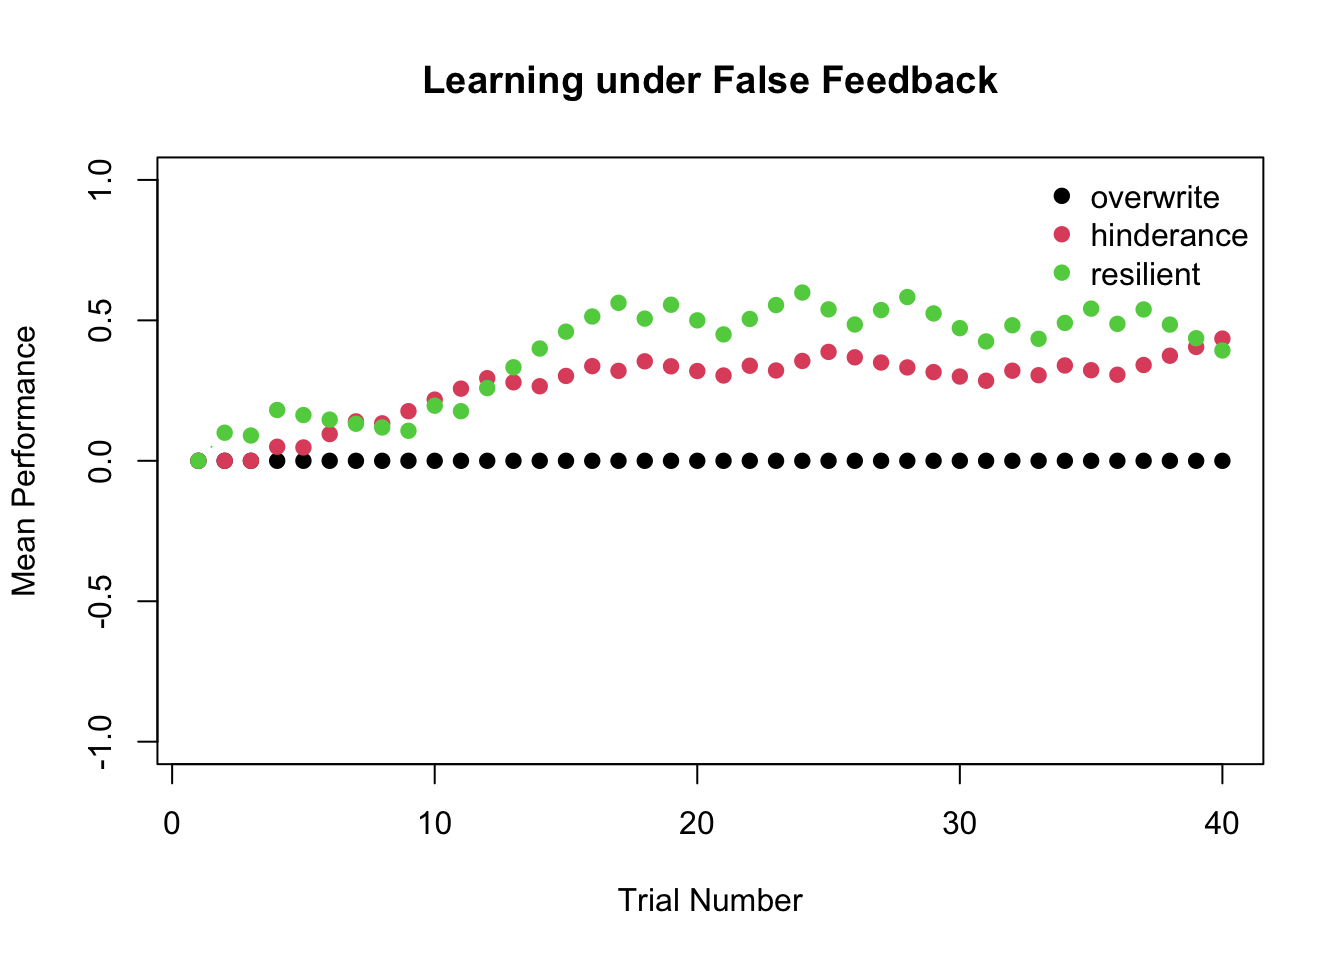
\includegraphics[bb=0in 0in 2.5in 2.5in, height=2.5in, width=2.5in]{Article/Figures/learning-curves-r.png}
    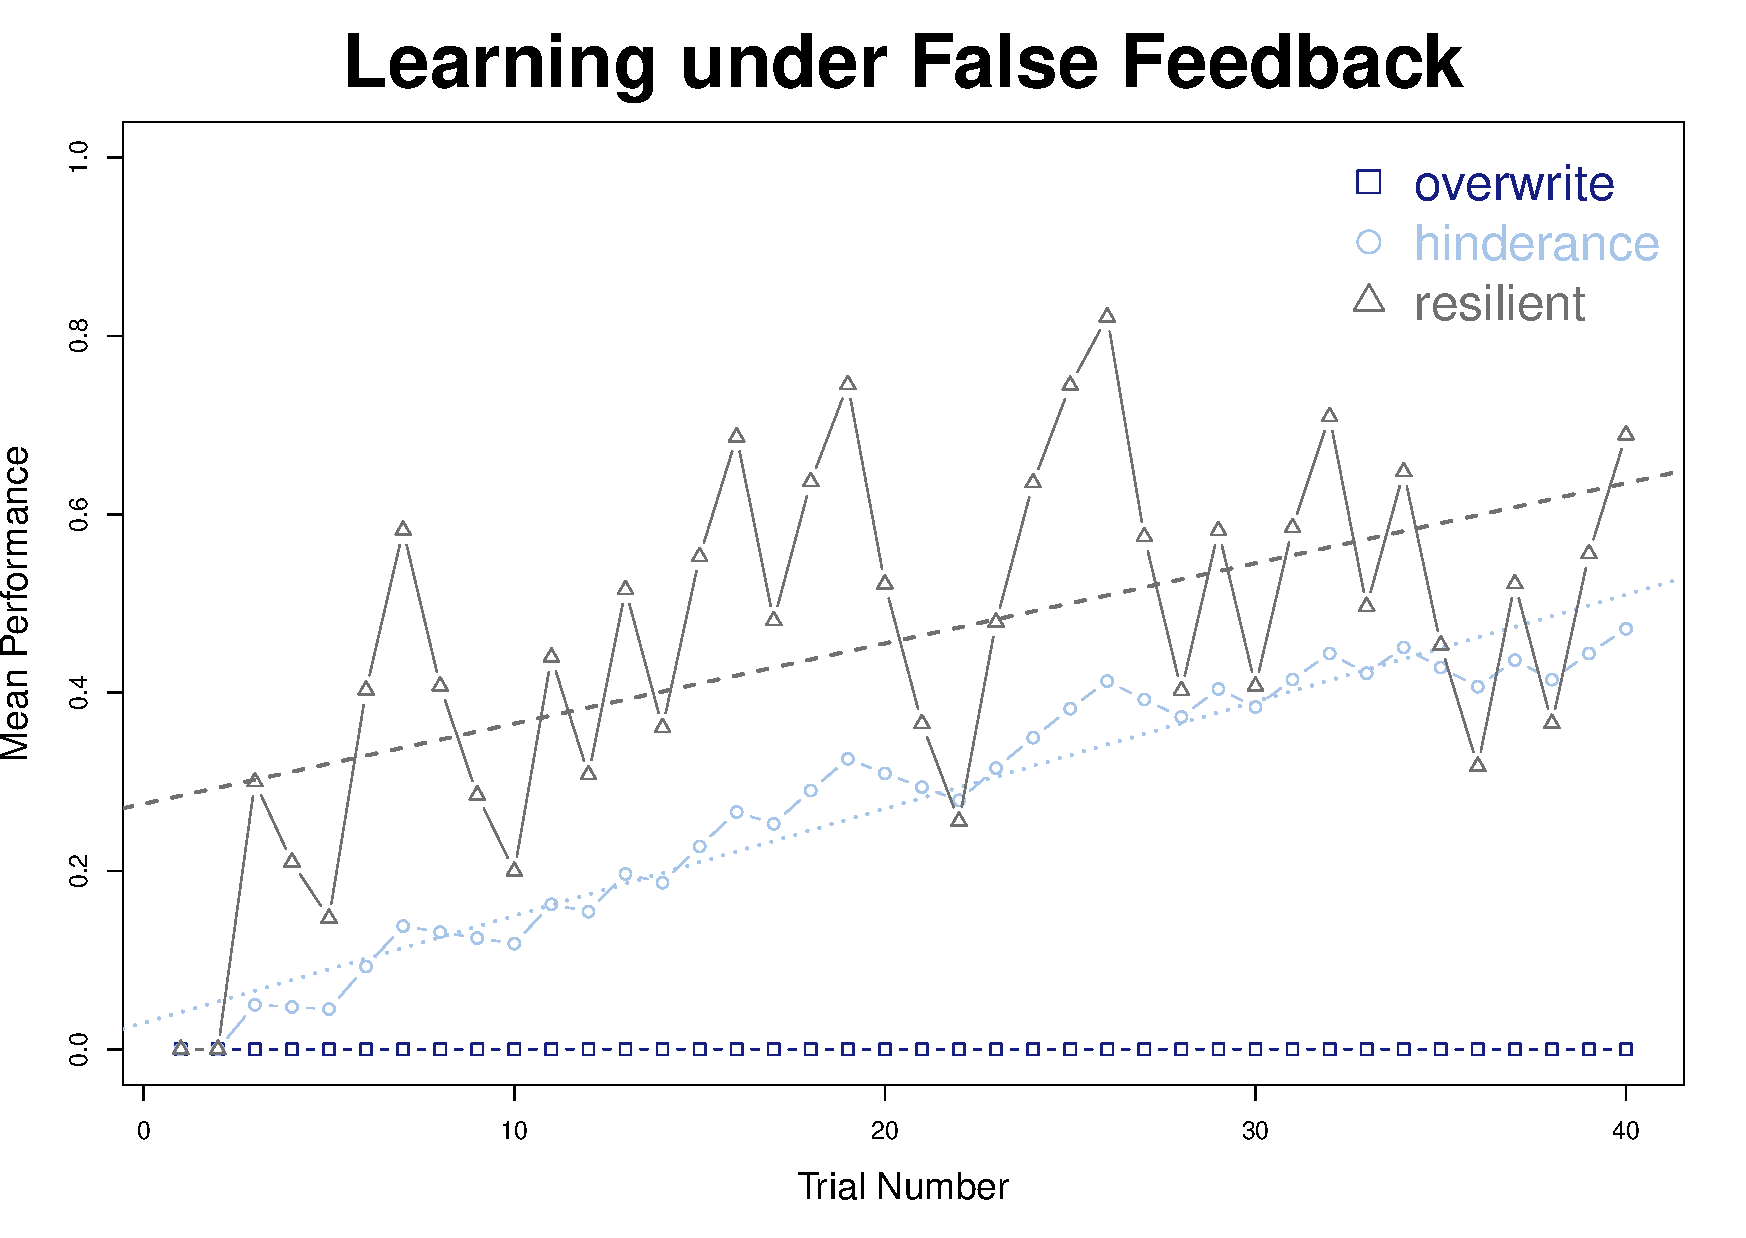
\includegraphics[scale=.6]{Figures/learning-curve.pdf}
    
    \label{fig:Figure1}
\end{figure}

\section{Methods}
\subsection{Participants}

Participants should be either only left-handed or right-handed. Gender should be balanced. If recruitment turns out to be difficult, the dominant side as well as gender should be collected as a control measure. Furthermore, as exclusion criteria data should not be collected from subjects, that can not move fingers in full range of motion, twist their wrists, have cerebral lesions which affect motor learning and are younger than 18 and older than 80 years old.

A small sample size of at least 4 subjects is required to find a sufficient statistical effect. The estimate has been computed with G*Power \parencite{erdfelder1996gpower}. The used parameters are, repeated measures main effects, an error probability of $\alpha$ = 0.05, 40 measurements, an estimated correlation for repeated measures of 0.50 and a desired power of 1 - $\beta$ = .9. The large effect of $\eta^2_p$ = .156 has been deduced from \citeauthor{Wei2009}'s finding in visual disturbance (\citeyear{Wei2009}).

Remuneration should be given adequately to the rules of the state (e.g. €12.96, Berlin TV Stud III). For fund acquisition, a duration of 30 minutes per participant is recommended.

\subsection{Experimental Set-Up}

Participants will lay inside the fMRI scanner with their hands (a) crossed and wrists twisted.

A 3D google has to be used to present the subject with a photorealistic virtual hand. The hands have to be in a sensible location to suggest limb ownership even when the hand is not actively moved.

To (implicitly) locate the body-selective EBA a short task has to be run prior to the experiment. A simple task could be to either let subjects move their hands vs observe non limb objects (see example in \cite{Limanowski2016}).

\subsection{Experimental Task}

In an experimental (and control) trial, the subjects will (a) observe a 3D representation of their hand for 2 s, followed by (b) an arrow which points to the finger they will have to move for 2 to 4 s. The arrow will (c) disappear and the subject is allowed to move the respective finger in full range of motion, for 4 s, without correction. To reduce temporal conditioning of the subject in the event-related task as to when the finger is allowed to move, a random jitter is added to step b. To prevent the subject from thinking too long prior each movement and to even out the participants pre-movement thinking duration each step c will be limited to these 4 s. The trial is cancelled if the participant does not move withing 1 s after trial-step on-set. After the task, the participant is presented with (d) fixation stimuli for 10 s before the next trial starts (inter-trial interval). While waiting, the participant verbally answers if they think that they have moved the correct finger and if the 3D hand representation has adequately moved the corresponding finger. One trial will take 18 - 20 s.

\subsection{Experimental Design}

For each participant, 4 runs, 10 trials each, will be carried out. Experimental (i.e. false visual feedback) and control trials (i.e. correct visual feedback) will be randomized over all trials. Randomization allows multiple conditions to appear after each other. Counter-balancing over all runs makes sure that learning is manipulated in the same manner in between participants. A one-minute fixation break will be made in between each run. The duration of the entire experiment will be 15 - 16.3 min and hold 40 in-between subject measurements of correct/incorrect responses.

Participants should complete a short training before data collection to get familiar to the task (e.g. two runs).

After the experiment, the participant should answer a short survey with a 6-point forced choice scale ranging from - 3 ("do not agree at all") to 3 ("fully agree"): (Q1) limb ownership: "Did you think the observed hand were your own?"; (Q2) vision/proprioception congruence: "I knew when the felt finger position was off the observed 3D finger movement", Personal vision vs proprioception preference: (Q3) "I could rely on my body sensation if I have moved the right finger."; (Q3) "I could rely on the visual feedback if I have moved the right finger.".

As collected data for each participant there will be for each trial a (a) performance measure: Finger movement (true/false), fMRI activations of the EBA and a manipulation check: (Q1) "Did you think you have moved the right finger?"; (Q2) "Did you think you have seen correct feedback?".

\section{Expected Results and Hypotheses}

\subsection{Expected Results}

The fMRI experiment bases its neural correlates on \parencite{Limanowski2016}. It is expected that false feedback, verbally reported by subjects, correlates with fMRI activity in the EBA. That is, that activity is significant in perceived correct feedback vs perceived false feedback (subjective feedback). Analogically, that activity is significant in experimental trials vs control trials (objective feedback).

Following these prerequisites, two hypotheses will be tested to answer the research question.

\subsection{Hypotheses}
\citeauthor{Limanowski2016} claims that sensory information is processed when proprioception and vision are congruent. That means that learning is affected when congruence is given. Learning in the proposed paradigm is determined with less behavioral errors, i.e. better performance over time. Mean prediction error should be lower after trials with correct feedback vs false feedback. Additionally, the \textit{resilient} learning rate parameter should not be able to predict the collected performance data significantly. The tested first hypothesis is:\\

\textbf{H1}: Congruence effects task performance (learning).\\

One of the two learning rate parameters, \textit{overwrite} and \textit{hinderance} are expected to explain a subject's performance best. How strong the effect of false visual feedback is on the learning rate is to be determined by the collected data. In any case better than the \textit{resilient} learning rate. The latter would falsify the general formulated second hypothesis: \\

\textbf{H2}: Visual input can outweigh proprioceptive information.

\section{Discussion}

The proposed experiment provides data to sheds light onto the learning curve under false visual feedback. The result will reproduce findings in neuronal EBA activation and show if the measure is valid also as behavioral learning measure.

A future experiment design should formulate a model that is closer to reality when concerning learning rates for finger movements. Considering all fingers of two hands as one motor primitive is too simple. In reality, the likelihood to move the correct finger in the paradigm is dependent on the side of the hand and also the distance between each finger. In other words it is more likely to confuse the contra- vs ipsilateral finger and the neighboring finger–i.e. index and middle vs index and pinky finger.

The experiment proposal falls in line with current literature of visuo-centric view of sensorimotor adaptation. Even though vision can outweigh proprioception, a model should respect cases where it is not the case. \citeauthor{Tsay2022} show, in their approach, a model that integrates proprioception in the process of sensorimotor adaption (\citeyear{Tsay2022}). A good model in the future should respect both senses, regardless of its inequality, so that it can explain more learning phenomena.

\printbibliography
\newpage

\section{Appendix}

\begin{table}
  \caption{Contingency Table Learning Outcomes}
  \label{tab:BasicTable}
  \begin{tabular}{@{}lrrrrrrrrr@{}}         \toprule
    &                      &                   &                 &                     &                     &                 & \multicolumn{3}{c}{Lerning rate param}        \\ \cmidrule(r){8-10}
  \# &  Instr.\tabfnm{a}      &   Moved\tabfnm{b} & Seen\tabfnm{c}  & Motor E.\tabfnm{d}  & Feedb. E.\tabfnm{e} & EBA \tabfnm{f}  & Res.\tabfnm{g}  & Hind.\tabfnm{h} & Overw.\tabfnm{i}\\ \midrule
  1 &  A                     &   A               & A               & 0                   & 0                   & 0               & 0               & 0                & 0 \\
  2 &  A                     &   A               & O               & 0                   & 1                   & 1               & 0               & 0                & 0 \\
  3 &  A                     &   O               & A               & 0                   & 0                   & 1               & .1              & -.05             & -.1 \\
  4 &  A                     &   O               & O               & 1                   & 1                   & 0               & .1              & .1               & .1 \\
  5 &  O                     &   A               & A               & 1                   & 1                   & 0               & .1              & .1               & .1 \\
  6 &  O                     &   A               & O               & 1                   & 0                   & 1               & .1              & 0                & 0 \\
  7 &  O                     &   O               & A               & 0                   & 1                   & 1               & 0               & -.05             & -.1 \\
  8 &  O                     &   O               & O               & 0                   & 0                   & 0               & 0               & 0                & 0 \\ \bottomrule
$\sum$ &                       &                  &                &                     &                     &                 & .4              & .1               & 0 \\ \bottomrule
  \end{tabular}
  \begin{tablenotes}[para,flushleft]
        {\small
            \textit{Note.} Some combinations are duplicate but listed for full comprehension.

            \tabfnt{a}Instructed finger to move.
            \tabfnt{b}The finger that has actually been moved.
            \tabfnt{c}The finger the subject observes in 3D goggles which moves.
            \tabfnt{d}Motor error.
            \tabfnt{e}Feedback error.
            \tabfnt{f}Activation in extrastriate body area.
            \tabfnt{g}Learning rate parameter according to \textit{resilient} rule.
            \tabfnt{h}Learning rate parameter according to \textit{hinderance} rule.
            \tabfnt{i}Learning rate parameter according to \textit{overwrite} rule. Learning rates divided by 10 fingers, to simulate individual learning each finger. A positive/negative value means beneficial/detrimental directed learning, zero means no learning.
            The letter \textit{A} represents any possible finger, \textit{B} represents any possible finger other than \textit{A}.
         }
    \end{tablenotes}
\end{table}


\subsection{Declaration of Independence}

Herewith I certify that I have prepared and written my thesis independently and that I have not used any sources and aids other than those indicated by me. \\
\mbox{}\\
\mbox{}\\
\mbox{}\\
\mbox{}\\
Antonio Amaddio, 12/12/2022


\end{document}


%% 
%% Copyright (C) 2019 by Daniel A. Weiss <daniel.weiss.led at gmail.com>
%% 
%% This work may be distributed and/or modified under the
%% conditions of the LaTeX Project Public License (LPPL), either
%% version 1.3c of this license or (at your option) any later
%% version.  The latest version of this license is in the file:
%% 
%% http://www.latex-project.org/lppl.txt
%% 
%% Users may freely modify these files without permission, as long as the
%% copyright line and this statement are maintained intact.
%% 
%% This work is not endorsed by, affiliated with, or probably even known
%% by, the American Psychological Association.
%% 
%% This work is "maintained" (as per LPPL maintenance status) by
%% Daniel A. Weiss.
%% 
%% This work consists of the file  apa7.dtx
%% and the derived files           apa7.ins,
%%                                 apa7.cls,
%%                                 apa7.pdf,
%%                                 README,
%%                                 APA7american.txt,
%%                                 APA7british.txt,
%%                                 APA7dutch.txt,
%%                                 APA7english.txt,
%%                                 APA7german.txt,
%%                                 APA7ngerman.txt,
%%                                 APA7greek.txt,
%%                                 APA7czech.txt,
%%                                 APA7turkish.txt,
%%                                 APA7endfloat.cfg,
%%                                 Figure1.pdf,
%%                                 shortsample.tex,
%%                                 longsample.tex, and
%%                                 experiment-proposal.bib.
%% 
%%
%% End of file `./samples/longsample.tex'.
